\documentclass[a4paper,12pt]{article}
\usepackage[margin=2cm]{geometry}
\usepackage[hidelinks]{hyperref}
\usepackage{graphicx}
\usepackage{float}
\usepackage{enumerate}
\usepackage{amsmath, amssymb}
\usepackage{mathtools}
\usepackage[utf8]{inputenc}
\usepackage{url}
\usepackage[nottoc,numbib]{tocbibind}
\usepackage{multicol}
\usepackage{caption}

\setlength\parindent{0pt}
\pagestyle{empty}
\numberwithin{equation}{section}

% Footnodes.
\makeatletter
\renewcommand\@makefntext[1]{\leftskip=2em\hskip-2em\@makefnmark#1}
\makeatother

% Abstract definition.
\renewenvironment{abstract}
 {\normalsize
  \begin{center}
  \bfseries \abstractname\vspace{-.5em}\vspace{0pt}
  \end{center}
  \list{}{%
    \setlength{\leftmargin}{20mm}%
    \setlength{\rightmargin}{\leftmargin}%
  }%
  \item\relax}
 {\endlist}

\def\changemargin#1#2{\list{}{\rightmargin#2\leftmargin#1}\item[]}
\let\endchangemargin=\endlist

% DRM macros
\newcommand{\drm}{\text{DRM}}
\newcommand{\nodrm}{\overline{\drm}}

% Whole game payoff macros (game_number, player number).
\newcommand{\artistpayoff}[2]{\pi_{#1, M_{#2}}}
\newcommand{\firmpayoff}[2]{\pi_{{#1}, F_{#2}}}

% Part game payoff macros.
\newcommand{\artistalbum}[2]{\pi_{#1, M_{#2}, A}}
\newcommand{\artistticket}[2]{\pi_{#1, M_{#2}, T}}
\newcommand{\firmalbum}[2]{\pi_{#1, F_{#2}, A}}
\newcommand{\firmticket}[2]{\pi_{#1, F_{#2}, T}}

% Derivative macros.
\newcommand{\deriv}[2]{\frac{d #1}{d #2}}
\newcommand{\doublederiv}[2]{\frac{d^2 #1}{d {#2}^2}}

% DRM influence on album demand.
\newcommand{\drminf}{(\psi \varepsilon - \gamma)}

% Ceiling commands.
\def\lc{\left\lceil}   
\def\rc{\right\rceil}

\begin{document}

% Title Page.
\begin{titlepage}
\begin{center}

\vspace*{3cm}
\Large
\begin{changemargin}{2cm}{2cm}
\begin{center}
\textbf{Game Theoretic Retrospective on DRM in the Music Industry}
\end{center}
\end{changemargin}

\vspace*{0.5cm}
\large
\textsc{Hugo Lhuillier}\\
Sciences Po\\[1.2em]
\textsc{Mitch Mastroni}\\
University of California, Santa Cruz\\[1.2em]
\textsc{Boonrith Pongrasamiroj}\\
Thammasat University\\[1.2em]
\textsc{Michael Sproul}\\
University of Sydney

\vspace*{1cm}
\begin{abstract}
Digital Rights Management, DRM, is a controversial mechanism for controlling the use of digital media. It once enjoyed popularity in the music industry, but has recently fallen into disuse and is now almost entirely absent. It persists in the video game industry however, and in this paper we seek to assess why this is the case, and how the market might evolve in the future. We provide a game theoretic model of a digital market for $m$ firms (product vendors) and $n$ artists. Consumers are modelled in the payoff functions of the players, and the firms can choose whether to enable DRM. Through backwards induction we derive the equilibria that exist for different settings of the game parameters, and apply quantitative data to explain the failure of DRM in the music industry.
\end{abstract}

\vfill

\normalsize
\textsc{Group 2}\\[1.2em]
\textsc{ECON 166A, Fall 2014}\\
University of California, Santa Cruz

\today

\end{center}
\end{titlepage}
\pagebreak

\section{Introduction}

All digital information is trivial to duplicate. From an MP3 file of a single song to an entire file system of digital assets and executables, an exact replica can be made with negligible monetary cost. With the advent of the internet, distribution of digital objects has too become trivial. Peer-to-peer file sharing has been utilized to illegally distribute a vast quantity of copyrighted material. The Recording Industry Association of America blames piracy for \$12.5 billion in economic losses every year \cite{fisher2007}.\\

As a reaction to file sharing, many industries adopted the use of digital rights management. The term digital rights management (DRM) broadly refers to a set of policies, techniques and tools that guide the proper use of digital content \cite{subramanya}. More specifically, DRM attempts to control the executing, viewing, copying, printing, and/or altering of digital works.\\

Over the past decade and a half, the music industry has implemented two types of DRM: one for audio CDs and another for music distributed through the internet. The DRM included on audio CDs became a commercial failure after Sony BMG's DRM that was introduced in 2005 was found to install a rootkit on the user's computer which caused a security vulnerability and eventually led to a recall of millions of CDs \cite{mcmillan}.\\

The primary focus of this paper is the use of DRM in internet music: music that was legally distributed online through stores such as the iTunes Store. This type of DRM restricts the use of the file, often limiting its use to a player provided by the store and linked to a specific user account. Although it was an industry standard in the first decade of the 21st century, some of the largest online music stores have moved away from DRM usage. In the case of Musicload.de, one of Europe's largest internet music retailers, openly expressed their disapproval of its usage in music \cite{vernik2011}.\\

Our goal is to model the relationship between the musicians (artists), record labels (firms), and listeners (consumers) and see how the equilibria relate to historical reality. We hope that by effectively modeling the decisions and payoffs around DRM in the music industry will allow us to create models for DRM usage in other industries that are accurate and predictive of future behavior.\\

This paper is constructed as followed. Section 2 review the existing
game theoretic literature about DRM systems. Section 3 presents the
game as well as the players' payoffs through a simple microeconomic
model. Section 4 derives the theoretical solutions for the game, while
section 5 applies actual empirical data to see how the model and the
game fit the actual music industry market. Section 6 presents the
possible extension of the game and gives some insights about their
solutions. Finally, section 7 analyzes the implications of our results
for the video game industry.

\section{Literature Review}

We begin with the paper that is interesting but simple called ``The DRM Game'' by Heileman G et al \cite{heileman2007}. It shows the game theoretical analysis of DRM as a simple extensive form game as well as a more advanced strategic form game. The first analysis consists of vendor and consumer playing a sequential move one-shot game where the consumer moves first. The consumer is, then, required to take an action on whether to purchase or illegally download. Vendor has an option to implement technological protection or not. The paper further shows that DRM could not be perfect, as in there will definitely be some leak even with the presence of technological protection thus allows file sharing to happen even in the case of DRM. More importantly, they focus on its subgame where, after both players choose the actions mentioned above, consumer decides to share or not to share files he or she obtains and vendor chooses whether to take a legal action against the consumer or not. The game needs to be solved with mixed strategy Nash equilibrium with the probability that vendor will take an action as low as around 0.4\% of the time. An important aspect that this paper gives us an insight about is that DRM is a negotiating game. In a repeated game where consumer and vendor play this game repetitively, the outcome is the same as a one-shot game. The equilibrium of this game has to be mixed. Both parties negotiate, indirectly through the repetitive nature of the game, until it is such that consumer’s behavior drives vendor to take an action against them meanwhile vendor’s action will force consumer to stop sharing. Hence, they conclude that the in the repeated game the equilibrium would be such that no matter the vendor imposes technological protection or not, the consumer will not share the content and the vendor will take action against piracy, even though they rarely do so.\\

In ``Who should own access rights? A game-theoretical approach to striking the optimal balance in the debate over Digital Rights Management'' by Yu-Lin Chang \cite{chang2007}, he approaches the problem in a very interesting way. The problem could not be solved by only looking at one aspect, namely, economics but need to be approached carefully on various sides. Chang introduces the concept of ``the notation of balance'' and argues that the way to solve this problem of implementing DRM is neither to give full restriction to the firm nor totally free access of the content to the public. He claims that it is about the right balance of the rights distributed between the two parties. While DRM in the past tended to limit the use of users who purchased the content, it fails miserably. At the same time, the era of free access when internet spread worldwide caused the information industry to lose a lot of money and was in trouble. The Nash equilibrium is when there is a correct amount of balance between the consumer’s right and the firm’s right to access to the content. Chang offers the solution that happens to be a prisoner’s dilemma where the Nash equilibrium is better for the society as a whole but is not the best for each player in the game.\\

There also is a paper which applies mathematics and computer programming to the analysis of how DRM works. Zhang, Pei, Ma, and Yang show in their paper ``Game-Theoretic Analyses and Simulations of Adoptions of Security Policies for DRM in Contents Sharing Scenario'' \cite{zhang2011} the method of constructing a payoff equation and matrices for provider and sharer. The game is shown as a simultaneous-move game. Later on, the game is evolved to dynamic and mixed game with two players, providers and sharers. They later on develop a simulation that simulates the repeated game with many sharers and providers as in the case of reality. The equilibrium occurs when the game is at all-enhanced security strategy. That is providers will forfeit all-general security, the old method of DRM which encrypt the files and make it very inconvenient to use in general, and turn to all-enhanced security strategy. They explain that it is a new method of DRM with higher security that enables users to share the content within their trusted devices, hence allows them to use the content as their wills within the acceptable constraint agreed by both providers and sharers.

\section{Model}
\subsection{Game Setting}

The DRM game is made of two categories of player, the record labels and the artists. The record labels are, with the artist, the major actors of the music industry market; indeed, a record label is a publishing company which ``coordinates the production, manufacture, distribution, marketing, promotion, and enforcement of copyright for sound recordings and music videos''\cite{klein2014}. Interestingly for this game is to note that there are a limited numbers of record labels in the current music industry market. According to the 2005 IFPI report, four firms were controlling more than three-fourth of the market in 2005; specifically, Universal Music Group had 28.8\% of the market, Sony Music Entertainment 21.1\%, EMI 14.1\%, and Warner Music Group 13.4\%.\\

The second category of players is the artist. Note that, even though the game represents the music market industry, consumers are not explicitly considered as players in the game, neither in the underlying model. Nonetheless, as DRM affect consumers' behaviors, either by forcing them to buy album by fighting illegal piracy, or by decreasing their willingness to pay for albums, consumers' preferences are incorporated into firms' and artists' profit function, as presented in the next section.\\

The whole game is divided into two games, with first a pricing game, and then the DRM game properly speaking.\footnote{
This duality is not consistent with the reality; in the real music industry market, firms decide simultaneously whether they want to implement DRM systems, and the price of their albums and concert tickets. However, in order to keep the model simple, we assumed that they were first fighting over the price of their products, and then taking a decision about DRM, maintaining those prices constant.
}\\

In the first game, the first players to move are the firms, competing against each other in order to maximize their profit by varying their album and concert tickets prices. When fixing its prices, a given firm does not know what the other firms are doing. Notice that prices have two effects in this game; first, by fixing higher prices than other record labels, a given firm appears as more profitable for artists. Therefore, more artists are likely to sign a contract with this record label, increasing ultimately its profit. However, higher prices imply in the meantime a lower demand for a given record label, potentially decreasing its profit.\\

Artists, observing prices fixed by record labels, decide then with which firms they want to sign a contract. For simplicity, they cannot quit the market, or be independent.\\

Follow this first game the DRM game, in which the album and concert ticket prices taken into account by the players are the ones determined in the first game. In this new game, firms choose first whether they want to enforce DRM systems in their product. A record label cannot decide to implement DRM only for some artists.  Enforcing DRM systems can have two opposite effects on a firm's profit. On one hand, by decreasing the number of illegal download, DRM increases the demand for album. On the other hand, consumers can have an aversion for album with DRM inside, triggering a decrease in the album demand. Moreover, artists can also dislike DRM since it could potentially decreases the exposure of their work, and, ergo, the number of people going to their concerts. The effect of DRM on firms' and artists' profit depends therefore on the relative impact of these two effects.\\

% EFG figure.
\begin{figure}[h]
\centering
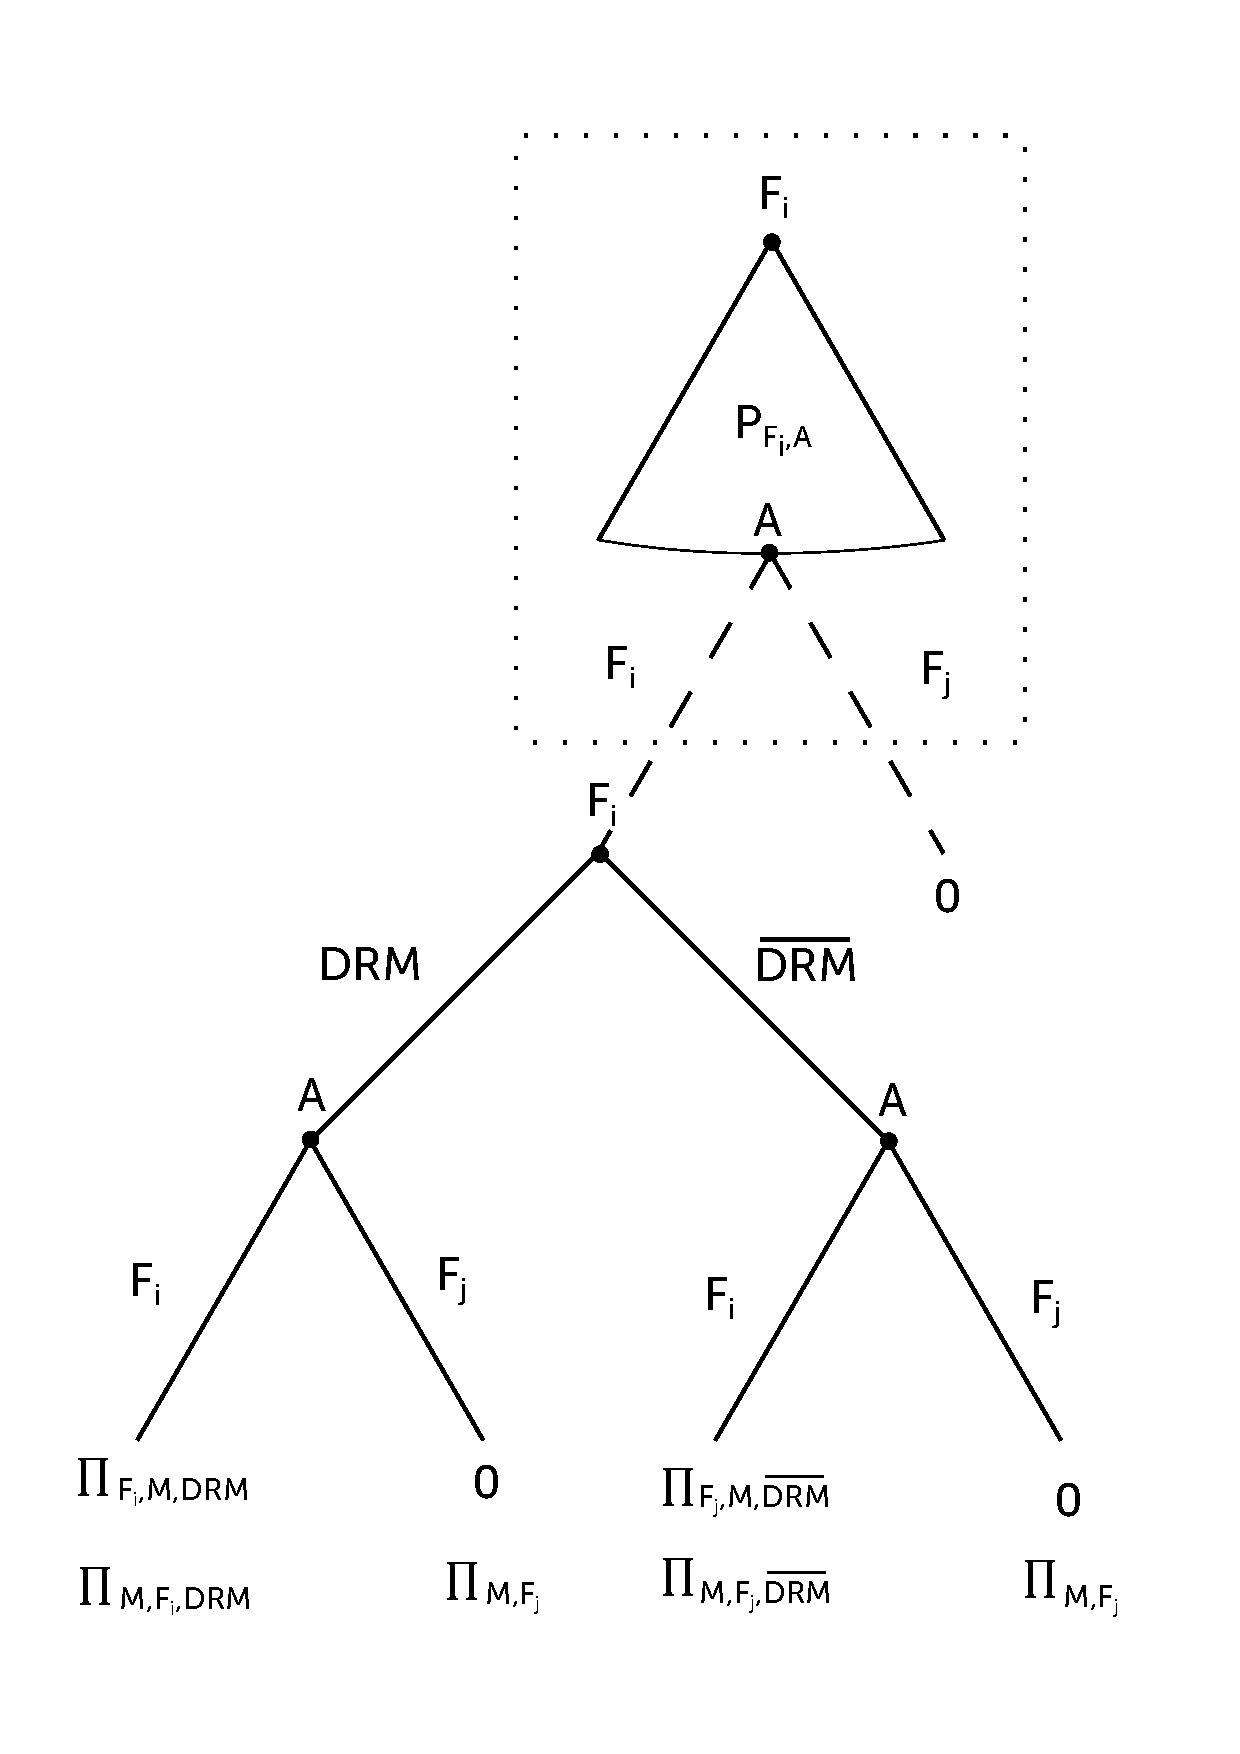
\includegraphics[width=12cm]{Graphics/GameTree.pdf}
\caption{Extensive Form Game for the Whole Game, from a Record Label's Perspective.}
\end{figure}

Figure 1 summarizes the previously described game configuration into an extensive form game. The dash box around the first two nodes represents the separation between the two games. Note that, for simplicity's sake, this figure is not the entire extensive form game, but the description of the game from a record label's point of view. Specifically, after deciding of a price, $P_{A, F_i}$, the artist can decide whether to go with this given record label, $F_i$, or any other firms, $F_j$, $i \ne j$. In the second game, the same label chooses whether enforcing DRM systems in its products, and the artist, once more, decides if he or she wants to go with this firm. If the artist opts for another firm, $F_j$, $F_i$'s profit is zero. If, on the contrary, the artist selects $F_i$, $F_i$'s payoff is positive, as described in the following section.

\subsection{Payoff Functions}

\subsubsection{Game 1: Pricing Game}

Firms are profit maximizer, that being true even in the music industry. Firms' payoff can therefore be described by a profit function such as $\pi_{F_i} = TR_{F_i} - TC_{F_i}$.\\

The record labels' revenues are made of the sales from the artists' albums under their label, tours and concerts from those same artists, and merchandising. For simplicity purpose, merchandising revenues are assumed to be constant for the four firms, so that firms' profits ultimately rely on revenues from album sales \& concerts \footnote{
A more realistic assumption is that merchandising revenues are a function of the albums and tickets sales – the more famous an artist is, the more album he or she sold, as well as tickets, the more merchandise products his or her fans purchase. In both case, record labels will try to maximize the quantity of albums and tickets sold to maximize the quantity of merchandise products.
}.\\

On the other side, record labels' costs are composed for more than two third of their total costs of marketing \& promotion expenditures, selling, general \& administrative expenses, and royalty payments. Because marketing \& promotion are not the topics of interest of this paper, they are assumed to be constant for the four firms, and, ergo, not taking into consideration into the model. Record labels' costs can be reduced to the payments of the artists under their label.\\

Therefore, the profit of a given firm, $F_i$, for a particular artist (musician) within the record label, $M$, can be describe as:
\begin{eqnarray}
\pi_{F_i, M} = \pi_{F_i, M, A} + \pi_{F_i, M, T}
\label{Eq:FirmTotalPayoff}
\end{eqnarray}  

Where $\pi_{Fi, M, A}$ is the record label's profit depending on the quantity of album sold for an artist $M$, and $\pi_{F_i, M, T}$ the record label's profit varying in function of the number of concert tickets sold for the same artist $M$. Specifically:
\begin{eqnarray}
\pi_{F_i, M, A} = (a_{A, M} - \sigma_{A, M} P_{A, M})(1 - \alpha_{A, M}) P_{A, M}
\label{Eq:FirmAlbumPayoff}
\end{eqnarray}

With $a_{A, M}$ a constant standing for the demand for the album of a given artist when its price is zero, $\sigma_{A, M}$ a constant expressing the variation of album sold induced by a marginal variation in album price, $P_{A, M}$ the price of an album $A$ for an artist $M$, fixed by the record label $F_i$, $a_{A, M}, \sigma_{A, M}, P_{A, M} > 0$, and $\alpha_{A, M}$ the album sharing rules determined by the record labels, $0 < \alpha_i < 1$. Equation $\eqref{Eq:FirmAlbumPayoff}$ is nothing more than a usual profit function, where the left-side of the equation represents the demand for albums - the demand being negatively related to the album price, and the right side of the equation describes the profit per album, namely the difference between the price of the album and its costs, assumed to be only made of the part of the price the record label is ready to giving up to the artist.\\

Similarly for the concert tickets profit:
\begin{eqnarray}
\pi_{F_i, M, T} = (a_{M, T} - \sigma_{M, T} P_{M, T})(1 - \alpha_{M, T}) P_{M, T}
\label{Eq:FirmTicketPayoff}
\end{eqnarray}

$a_{M, T}$ is a constant portraying the demand for concert tickets of a given artist when its price is zero, $\sigma_{M, T}$ is a constant precising the variation of concert ticket sold triggered by a marginal variation in concert ticket price, $P_{M, T}$ is the price of a concert ticket, $a_{M, T}, \sigma_{M, T}, P_{M, T} > 0$, and $\alpha_{M, T}$ the concert ticket sharing rules, also determined by the record labels, $0 < \alpha_i < 1$.\\

Substituting \eqref{Eq:FirmAlbumPayoff} and \eqref{Eq:FirmTicketPayoff} into \eqref{Eq:FirmTotalPayoff} yields the following record label’s profit function for one of its artists, $M$:
\begin{eqnarray}
\pi_{F_i, M} = (a_{M, A} - \sigma_{M, A} P_{M, A})(1 - \alpha_{M, A}) P_{M, A} +
	(a_{M, T} - \sigma_{M, T} P_{M, T})(1 - \alpha_{M, T}) P_{M, T}
\end{eqnarray}

To simplify this model, the albums and concert tickets prices are presumed equal for all artists within a record label, as well as the album and concert tickets sharing rules \footnote{
These assumptions are empirically not true; however, this paper is interested in looking at how competition between firms shapes the decisions about whether or not implementing DRM systems. In that sense, even though prices are obviously different among artists within a record label, one can consider $P_{M, A}$ and $P_{M, T}$ as the mean of all different possible prices of albums and concert tickets within a record label. The same explanation can be provided for $\alpha_A$ and $\alpha_T$ equal for all artists within a firm.
}.

Moreover, it is assumed that the album and tickets demand when the price is zero, the price elasticity of album and concert tickets, and the album and concerts sharing rules are equal for the four labels, such that $a_{M, A} = a_A$. Additionally, the concert ticket price can be expressed as a function of the album price:
\begin{eqnarray*}
P_{i, T} = k P_{i, A}
\end{eqnarray*}

Where $k$ is a constant defined as the average concert ticket price over the average album price, $k > 0$. Adding altogether those changes shows the following record label’s profit function for a given artist, $M$:
\begin{eqnarray}
\pi_{F_i, M} = (a_A - \sigma_A P_{F_i, A})(1 - \alpha_A) P_{F_i, A} +
	(a_T - \sigma_T k P_{F_i, A}) (1 - \alpha_T) k P_{F_i, A}
\end{eqnarray}

From here, record label’s profit function for any artist being the same for all artists under contract with it, its total profit function is the sum of the per artist profit:
\begin{eqnarray}
\pi_{F_i} = l_{F_i} (a_A - \sigma P_{F_i, A})(1 - \alpha_A) P_{F_i, A} +
	(a_T - \sigma_T k P_{F_i, A})(1 - \alpha_T) k P_{F_i, A}
\end{eqnarray}

$l_{F_i}$ standing for the number of artist under contract with the record label, $l_{F_i} \in [0, n]$, such that $\sum_{i = 1}^m l_i = n$, $n$ being the total number of artists in the music industry market, $m$ being the number of firms (in our case, 4).\\

The other players’ payoffs, namely the artists’ payoffs, are defined similarly. Specifically, their album and concert demands are the same as the record labels’ ones, and their profit per unit are the complement of the record label’s revenue, i.e. the share of the concert ticket or album price the record label accept to give to them, $\alpha P_{F_i, A}$ or $\alpha_T k P_{F_i, A}$. Finally, making an album or putting on a concert is not without costs to the artist, so the constants $C_A$ and $C_T$, where $C_A, C_T > 0$,  encode the cost of producing an album and a concert series respectively. Those two finals parameters are assumed to be fixed cost defined exogenously\footnote{
This assumption is consistent with the reality of the music market industry since, most of the time, artists sign a contract with a record label stipulating a priori how much the production of an album will cost to them, and this cost does not evolve with the number of album sold.
}. Formally, the payoff function of a given artist, $M$, is given by:
\begin{eqnarray}
\pi_M = (a_A - \sigma_A P_{F_i, A})\alpha_A P_{F_i, A} - C_A
	+ (\alpha_T - \sigma_T k P_{F_i, A}) \alpha_T k P_{F_i, A} - C_T
\end{eqnarray}

This formal description of the model is useful to define the player’s strategy set. The four firms, $F_i$, playing first, chooses $P_{F_i, A} > 0$, followed by the artists, signing a contract with a record label $F_i, i \in [1, m]$, where $m = 4$. Because all artists have the same payoff function, a representative artist is designated as the only player for the artist category. 

\subsubsection{Game 2: DRM Game}

The second game studies whether record labels have incentives to implement DRM in their products. The players’ payoff functions are mainly based on the same framework as the first game, except that $P_{F_i, A}$ is now considered as a constant, and no longer as an independent variable.\\

Formally, recalling that a firm’s album and a firm’s ticket concert profit are:
\begin{eqnarray}
\pi_{F_i, A} = l_{F_i} (a_A - \sigma_A P_{F_i, A})(1 - \alpha_{F_i, A}) P_{F_i, A}\\
\pi_{F_i, T} = l_{F_i} (a_A - \sigma_A P_{F_i, A})(1 - \alpha_{F_i, T}) k P_{F_i, A}
\end{eqnarray}

The new payoff function is defined as:

\begin{eqnarray}
\firmpayoff{2}{i} = \firmalbum{1}{i} (D_A) + \firmticket{1}{i}  (D_T) - C_{\drm}
\label{Eq:FirmTotalPayoffDRM}
\end{eqnarray}

Where $D_A$ and $D_T$ are respectively the impact of DRM on the album and ticket concert profit, and $C_{\drm}$ stands for the cost of implementing DRM systems. Specifically:
\begin{eqnarray}
D_A = 1 + \delta \drminf
\label{Eq:DA}
\end{eqnarray}

With $\delta$ a binary variable, $\delta \in \{0, 1\}$, equal to one when DRM systems are enforced, $\psi$ the number of illegal download for a record label, and $\gamma$ the consumers’ disutility of purchasing an album with DRM in it, $\psi > 0, \gamma \geq 0$. DRM can indeed be viewed as a constraint from the consumer’s point of view, reducing his or her willingness to pay for a given album. Finally, $\varepsilon$ represents the effectiveness of DRM to fight illegal piracy, $0 \leq \varepsilon \leq 1$, such that if $\varepsilon = 1$, DRM systems are extremely effective and illegal download no longer exists. Therefore, $\drminf$ describes the tradeoff record labels are facing when they are deciding whether they should implement DRM systems.\\

Similarly:
\begin{eqnarray}
D_T = 1 - \delta \theta
\label{Eq:DT}
\end{eqnarray}

Where $\theta$ is the number of tickets non-sold due to the presence of DRM on firms’ products, coming both from the fact that consumers do not want to go to concerts of artist who have DRM on their music and from the fact that the music of artists with DRM systems can be less spread due to more difficulties to illegally download the product, generating therefore less fans, $\theta > 0$.\\

Finally, implementing DRM systems has a cost:
\begin{eqnarray}
C_\drm = \frac{\rho}{l_{F_i} + 1}
\label{Eq:CostDRM}
\end{eqnarray}

$\rho$ portraying the cost of DRM, $\rho > 0$. Implicit in this cost function is that economies of scale exist, such that, for a given value of $\rho$ for a given firm, the cost of implementing DRM will decrease as the number of artists within this label increases.\\

Equation \eqref{Eq:FirmTotalPayoffDRM} can be seen in terms of percentage. If a firm decides to not implement DRM, then delta equals zero, and its payoff, $\firmpayoff{2}{i}$, is identical to the one derived in the previous game (100\%). If, on the contrary, a record label chooses to go for DRM, then its profit evolves by $\drminf$, depending on the effectiveness of DRM and the way consumers dislike DRM, $\drminf$ defining a percentage of the previous profit, possibly greater or smaller than 100\%\footnote {
Section \ref{Sec:Estimates} estimates those parameters and substitutes them into the profit functions, which can help to better understand the new payoff function if this is not already the case.
}.\\

In order to not add further complexity to this model, $\gamma$, $\psi$ and $\varepsilon$ are assumed to be constant and equal for all firms. Of particular interest for our topic, $\varepsilon$ is defined exogenously, such that record labels have no control over the effectiveness of DRM. This strong assumption is discussed in section \ref{Sec:Extensions}, where possible extensions of the model are presented.\\

Substituting \eqref{Eq:DA}, \eqref{Eq:DT} and \eqref{Eq:CostDRM} into \eqref{Eq:FirmTotalPayoffDRM} yields:
\begin{eqnarray}
\firmpayoff{2}{i} = l_{F_i} \left[
	(1 + \delta \drminf) \firmalbum{1}{i} +
	(1 - \delta \theta) \firmticket{1}{i}
\right]
- \delta \left( \frac{\rho}{l_{F_i} + 1} \right)
\end{eqnarray}

Regarding the representative artist’s payoff, the impact of DRM on his or her profit is the same as the one for the record labels. Formally, his or her new payoff function is given by:
\begin{eqnarray}
\artistpayoff{2}{i} = (1 + \delta \drminf) \artistalbum{1}{i} - C_A +
						(1 - \delta \theta) \artistticket{1}{i} - C_T
\end{eqnarray}

Once more, this formal description is useful to derive players’ strategy set. Firms, acting first, choose $\delta \in \{0, 1\}$, followed by the representative artist, deciding to sign a contract with one of the four labels, $F_i$, $F_i \in \{F_1, F_2, F_3, F_4\}$.

\section{Solutions}

\subsection{Game 1: Pricing Game}

To solve the pricing game, we considered the optimal price desired by the artists. All the artists have the same payoff function, $\artistpayoff{1}{i}$, which depends on the continuous variable $P_A$ and no discretely valued variables. Therefore it is possible to maximise $\artistpayoff{1}{i}$ using simple calculus. Given an artist-optimal value of the album price, $P_A^*$, we prove that the firms must all set this price in any Nash Equilibrium utilising pure strategies.\\

Imagine a situation where the firms have agreed on prices such that the highest price chosen by a firm is $P_A^- < P_A^*$. In this case, all firms not already choosing $P_A^-$ have a best response to increase their price to $P_A^-$ in order to make them indistinguishable from the top firm(s), which would otherwise take the business of all the artists. Artists care only about getting as close to $P_A^*$ as possible, and will always choose the firm that offers the closest price. To this end, the firms all have a best response to increase their price to get closest to $P_A^*$. With this pressure applied from the upwards direction as well, it's clear that the only equilibria will have all of the firms setting their price at $P_A^*$.\\

With all the firms offering the same price, the artists have no way to distunguish them, and can choose arbitrarily without destroying the equilibria. Given that each of the $n$ artists has a choice of $m$ firms, this gives rise to $m^n$ Nash Equilibria in the pricing game.\\

$P_A^*$ can be found by maximising $\artistpayoff{1}{i}$:
\begin{eqnarray*}
\artistpayoff{1}{i} & = & (a_A - \sigma_A P_A)\alpha_A P_A + (a_T - k \sigma_T P_A) k \alpha_T P_A\\
\deriv{\pi}{P_A} & = & a_A \alpha_A - 2 \alpha_A \sigma_A P_A + k a_T \alpha_T - 2 \alpha_T \sigma_T k P_A\\
\doublederiv{\pi}{P_A} & = & -2(\alpha_A \sigma_A + \alpha_T \sigma_T) < 0 \Rightarrow \text{maximum}
\end{eqnarray*}

Solving $\deriv{\pi}{P_A} = 0$ yields:
\begin{eqnarray}
P_A^* = \frac{\alpha_A a_A + k \alpha_T a_T}{2(\alpha_A \sigma_A + k \alpha_T \sigma_T)}
\end{eqnarray}

\subsection{Game 2: DRM Game}

The solution to the DRM game has a similar structure to that of the pricing game. Once again, the artists control the behaviour of the firms, and are free to choose between them. The difference is that the DRM game is paramaterised by a number of constants: $\psi$, $\varepsilon$, $\gamma$ and $\rho$, which generate several types of systems. In this section we explore the nature of equilibria in these different systems.\\

Given the payoff function for the artists as follows, note that the artists will have a strict preference for DRM or $\overline{\text{DRM}}$:
\begin{eqnarray*}
\artistpayoff{2}{i} = (1 + \delta (\psi \varepsilon - \gamma)) \artistalbum{1}{i} + (1 - \delta \theta) \artistticket{1}{i}
\end{eqnarray*}

This follows from the fact that the payoff from the first game is fixed, and that $\delta$ is a binary variable. Comparing the payoff with DRM to the payoff without, there are three possiblities: either DRM is favourable, $\nodrm$ is favourable, or the payoffs are equal, in which case the artists are ambivalent.\\

First consider the two cases where the payoffs are different. In these cases, the best response of the firms is to set $\delta$ according to the artists' preference. It is impossible to have an equilibrium where the firms set $\delta$ against the artists' preference, as this would result in one firm deviating and stealing the entire market. Hence the only possible equilibria involve all the firms setting $\delta$ in the way that is optimal for the artists. As before, the artists then have no way to differentiate the firms and can choose between them freely, for a total of $m^n$ Nash Equilibria in pure strategies.\\

This is not quite the whole story however, as the firms also pay a cost for implementing DRM, and may be forced to disable DRM if this cost is prohibitive. Accumulating more artists reduces the cost of DRM, and hence for each system, there is a number of players $\eta$, such that firms with $\eta$ or more players are better off if they implement DRM. Computing the value of $\eta$ is done by equating the two firm payoffs:
\begin{eqnarray*}
\firmpayoff{2}{i}(\delta = 1, l_i = \eta) & = & \firmpayoff{2}{i}(\delta = 0, l_i = \eta)\\
\eta \left[\left(1 + \delta \drminf\right) \firmalbum{1}{i} + (1 - \delta \theta) \firmticket{1}{i}\right] - \frac{\rho}{\eta + 1} & = & \eta (\firmalbum{1}{i} + \firmticket{1}{i})
\end{eqnarray*}

Solving for (positive) $\eta$ yields:
\begin{eqnarray}
\eta & = & \lc \frac{-1 + \sqrt{1 + 4 x}}{2} \rc \\
\text{where } x & = & \frac{\rho}{\drminf \firmalbum{1}{i} - \theta \firmticket{1}{i}} \nonumber
\end{eqnarray}

We are now in a position to classify some more system behaviour. If $\eta = 1$, then it is always beneficial for firms to implement DRM, given a fixed value of $l_i > 0$. We say that the DRM is \textit{strongly firm-beneficial}. At the other extreme, if $\eta > n$, then firms are worse-off implementing DRM for a fixed choice of $l_i > 0$, and we say that the DRM is \textit{strongly firm-detrimental}. Note that the presence of strongly beneficial or strongly detrimental DRM is not sufficient to predict what the firms will choose, due to the market effect introduced by the artists. As explained above, if artists prefer one DRM state to another, firms must choose that state to avoid losing the entire market. The exception to this is firms with no artists, which must always choose $\nodrm$, to avoid a negative payoff. The resulting dynamics are best captured by an exhaustive enumeration of possible scenarios.
\begin{itemize}
\item Artists prefer DRM.
	\begin{itemize}
	\item DRM is strongly firm-beneficial ($\eta = 1$): All firms with associated artists enable DRM. Any configuration of this form is a Nash Equilibrium.
	\item DRM is strongly firm-detrimental ($\eta > n$): As long as the firm payoff for implementing DRM is not negative, all equilibria involve firms with non-zero $l_i$ enabling DRM due to the market effect, and firms with $l_i = 0$ disabling DRM to avoid negative payoffs. If the firm payoff is negative for values of $l_i > l_i^* > 0$, then the system is \textit{degenerate}. In the interests of brevity we don't consider such systems here.
	\item DRM is firm-moderate ($1 < \eta \leq n$): Nash Equilibria in this case are comprised of some firms with DRM enabled and $l_i \geq \eta$, and others with DRM disabled and $l_i = 0$.
	\end{itemize}
\item Artists prefer no DRM.\\
In this case, the firm preference is irrelevant. At equilibrium, all firms disable DRM and artists associate freely.
\end{itemize}

In the case where artists are ambivalent to DRM, equilibria are characterised by some firms with DRM enabled and $l_i \geq \eta$, and others with DRM disabled and $\eta < \eta$. This is similar to the case where artists prefer DRM and DRM is firm-moderate, except that firms without DRM can posess artists at equilibrium.\\

Finally, we come to describing the parametrisations that cause artists to prefer one DRM state over another. It would take many pages to quantify the influence of all three parameters influencing artists ($\psi, \varepsilon$, $\gamma$ and $\theta$), so we concern ourselves only with $\varepsilon$ - the effectiveness of DRM in preventing piracy - as it is the least well known. In the next section we provide real-world estimates of the other parameters.\\

To compute the critical value of $\varepsilon$ at which artist preferences flip, we solved the following inequation involving the payoffs with and without DRM:
\begin{eqnarray*}
\artistpayoff{2}{i}(\delta = 1) & > & \artistpayoff{2}{i}(\delta = 0)\\
(1 + \delta \drminf) \artistalbum{1}{i} + (1 - \delta \theta) \artistticket{1}{i} & > & \artistalbum{1}{i} + \artistticket{1}{i}
\end{eqnarray*}

Solving for $\varepsilon$ we have that DRM is artist-beneficial when:
\begin{eqnarray}
\varepsilon > \frac{1}{\psi} \left( \frac{\theta \artistticket{1}{i}}{\artistalbum{1}{i}} + \gamma \right)
\label{Eq:EpsilonStar}
\end{eqnarray}

When $\varepsilon$ is equal to the term on the right, which we shall call $\varepsilon^*$, the payoffs are equal and the artists are DRM ambivalent. Combined with the characterisations from above, and values for $\psi, \gamma, \theta$ and $\rho$ this allows us to predict the equilibrium behaviour of a DRM system where $\varepsilon$ is uncertain.\\

Conceptually, the tension between artists and firms over DRM is a consequence of varying valuations of albums and concerts, and the impact that DRM has on both. Whilst it is possible (and even likely), for DRM to have little impact on concerts, this can have a profound impact on the dynamics of the game if arists receive more of their revenue from concerts ($\alpha_T \gg \alpha_A$), and therefore feel the impact of DRM stronger than the firms. Conversely, firms are more likely to be negatively effected by DRM if $\drminf$ is large, and firms draw most of their revenue from album sales ($\alpha_T \ll \alpha_A$). This interaction is discussed further in section \ref{Sec:Estimates}.

\section{Estimation of Parameters} \label{Sec:Estimates}

\subsection{Estimation of Empirical Data for the Music Industry}

This section assigns values to the parameters previously presented,
in accordance with empirical data, so that it is possible to observe
whether the solutions derived in the previous section are consistent
with the real music industry market. Knowing that the price elasticity
of the album demand is 2.8\% \cite{gast2002}, the average slope of
the album demand function has been estimated to 0.288\footnote{
The estimation method is presented in the appendix, section \ref{Sec:SigmaEstimates}.
}:
\begin{eqnarray*}
\sigma_{A}=0.288
\end{eqnarray*}

Similarly, the slope of the concert tickets demand function, knowing
that the demand for concerts is almost inelastic in prices \cite{courty2009}, has been estimated to 0.01\footnote{
The estimation method is presented in the appendix, section \ref{Sec:SigmaEstimates}.
}:

\begin{eqnarray*}
\sigma_{T}=0.011
\end{eqnarray*}

The sharing rules parameters are easier to estimate, several studies
and data being available. Specifically, according to David McCandless \cite{mccandless2010}, the artists got as much as \$0.94 when the
album priced \$9.99 is sold and they receive \$0.09 for a track download
worth \$0.99. Hence, $\alpha_{A},$ the share amount of what the artists
get, can be estimated as:
\begin{eqnarray*}
\alpha_{A}=0.1
\end{eqnarray*}

Even though the range of the concert ticket sharing rule is larger
than the one of the album sharing rule, the former evolving within
the spectrum 65\%-90\% depending on the artist and the agreement between
the two (or more) parties, the share that the artists get from a concert
ticket sold is on average 74\% of its price \cite{michael2011}:

\begin{eqnarray*}
\alpha_{T} = 0.74
\end{eqnarray*}

Estimating the coefficient relating album and concert ticket prices
through regression analysis is complex since the standard deviation
of album prices is way smaller, almost nonexistent, compared to the
standard deviation of concert ticket prices. Instead, album and concert
ticket prices have been aggregated, and these parameters have been estimated
as the average concert ticket price over the average album price,
such that:

\begin{eqnarray*}
k=3.4
\end{eqnarray*}

Finally, $a_{A}$ and $a_{T}$ remain unspecified, as well as $C_{A}$ and
$C_{T}$, due to lack of data available. The next section fixes arbitrarily
those constants in order to make the result of this paper clear and
straightforward for everyone. Hence, the new payoff function can be
restated as:

\begin{eqnarray*}
\pi_{F_{i}} & = & l_{F_{i}}((a_{A}-0.288P_{A,F_{i}})(0.9P_{A,F_{i}})+(a_{T}-0.037P_{A,F_{i}})(0.88P_{A,F_{i}}))\\
\pi_{M_i} & = & (a_{A}-0.288P_{A,F_{i}})(0.1P_{A,F_{i}})-C_{A}+(a_{T}-0.037P_{A,F_{i}})(3.06P_{A,F_{i}})-C_{T}
\end{eqnarray*}

Regarding the second game, the removal of DRM increases the digital
sales by 10\% according to Laurina Zhang \cite{zhang2014}, implying
that the disutility of DRM should be rounded up to 10\%, or:
\begin{eqnarray*}
\gamma=0.1
\end{eqnarray*}

Moreover, following the estimation made by the research from the NPD
Group, Inc., in 2009 \cite{npd2009}, only 37\% of the songs attained
by US consumers were paid for, implying that 63\% of those were illegally
obtained. Removing entirely illegal download, if DRM systems were
perfectly effective, would then increase the demand for album by 70\%.
Ergo:
\begin{eqnarray*}
\psi=1.7
\end{eqnarray*}

Even though clear and straightforward empirical data about the negative
impact of DRM on ticket concerts sales have not been found, this paper
assumes that $\theta=0.05$. Note that, besides capturing the direct
effect of DRM on concerts, this parameter could also represents the
various indirect negative impact of the presence of DRM on artists’
payoffs; one of them could for instance be some artists’ ideals about
the public sharing of albums\footnote{
For instance, The Grateful Dead allowed their fans to record their
concerts and then to distribute thoserecords to other people. Even
more, some of their albums were totally free.
}.\\

Finally, in addition to previous unestimated parameters,$\rho$ is
not defined due to lack of empirical information. Adding together
all those new estimations brings new payoff functions, defined as:
\begin{eqnarray*}
\pi_{F_{i}}=l_{F_{i}}((1+\delta(1.7\varepsilon-0.1))(\pi_{F_{i},A})+(1-\delta0.05)(\pi_{F_{i},T}))-\delta(\frac{\rho}{l_{Fi}+1})\\
\pi_{m}=(1+\delta(1.7\varepsilon-0.1))(\pi_{m,A})-C_{A}+(1-\delta0.05)(\pi_{m,T})-C_{T}
\end{eqnarray*}


From here, the solutions derived in the previous section can be adjusted
to empirical data, allowing to observe whether the critical value
of $\varepsilon$ is achievable.

\subsection{Equilibria in the Music Industry}

We are finally in a position to analyse the music industry in terms of our model. Unfortunately, with the ``realistic'' parameters of the previous section, our model falls apart. We discovered this too late before the deadline to ammend the model, so instead present a model with an altered set of paramaters, to highlight the kind of analysis we would like to do.\\

Firstly, the paramaters. It was found that values of $k > 2$, in combination with values of $a$ and $\sigma$ within an order of magnitude of each other (to produce $P_A \approx 10$), cause the payoff for the artists to be negative, $\artistpayoff{1}{i} < 0$. This is unreasonable as it fails to reflect reality, and more worringly, propogates negative payoffs throughout the model which undermine the incentive for firms to attract artists. To remedy this problem, we altered the parameters as follows:

\begin{eqnarray*}
k & = & 1.8\\
\sigma_A & = & \sigma_T = 4\\
a_A & = & 100\\
a_T & = & 150\\
C_A & = & C_T = 2
\end{eqnarray*}

These parameters, whilst unrealistic, at least provide a price close to \$10, $P_A = 18.3$, and positive payoffs for the artists, $\artistalbum{1}{i} \approx 104$. All other paramaters were set at their values from the first part of this section.\\

Using \eqref{Eq:EpsilonStar} to compute the critical value of $\varepsilon$ yields $\varepsilon^* \approx 0.0829$, meaning that DRM only has to be 8.29\% effective in converting pirates to be econmically viable for artists. Unfortunately, the model is too broken to allow a sensible computation of $\eta$. However, given the lack of DRM in the music industry, and the fact that the only equilibria that permit this occur when artists prefer $\nodrm$, our model predicts the true value of $\varepsilon$ to be less than $\varepsilon^* \approx 0.0829$. Although this figure is quite low, it is within the realm of possibility - perhaps DRM really is woefully ineffective. Further improvements to the model would be required to make a stronger judgement.

\section{Extensions to the Model} \label{Sec:Extensions}

This section presents and discusses several developments of the DRM
game model, all linked with the effectiveness of DRM, $\varepsilon$,
in order to increase the fitness of model with the actual music market
industry. Since here, $\varepsilon$ has been assumed to be (a) constant
(b) defined exogenously, so that a firm has no control over its value
(c) known by the firms and the artists. Those three simplifications
are presently discussed and reconsidered one by one. The new games
hereby created will not be solved formally, even though insights about
the solutions will be provided.\\

There is first no reason to consider $\varepsilon$ as a constant.
Consumers, by getting used to DRM, can improve their knowledge on
how to pirate products with DRM inside; on the other side, firms,
by investing in Research \& Development, can increase the effectiveness
of DRM. Therefore, instead of taking the value of $\varepsilon$ as
defined exogenously, the effectiveness of DRM can depend on the amount
of money invest in DRM technology.\\

Taking into account these previous remarks, a game with new payoff
functions can be derived. Precisely, the record labels’ payoff function
are now given by:
\begin{eqnarray*}
\pi_{F_{i}}=l_{F_{i}}((1+\delta(-0.1+1.7\varepsilon))(\pi_{F_{i},A})+(1-\delta0.05)(\pi_{F_{I},T}))-\delta(\frac{\rho}{l_{i}+1})
\end{eqnarray*}

where $\varepsilon=f(\rho)=k_{1}(1-e^{-k_{2}\rho})$.\\

Figure \ref{Fig:EpsilonEvolution} presents how the effectiveness of DRM evolves depending on
the investment on DRM. Namely,$\varepsilon$ is increasing at a decreasing
rate with$\rho$, specifying that increasing the amount of money investing
in DRM systems allow to increase its effectiveness, even though this
improvement becomes smaller and smaller as$\varepsilon$ becomes larger.
Besides having a new payoff function, records label also have a new
strategy set; specifically, firms need now to choose whether or not
implementing DRM,$\delta$, and the amount of money investing in DRM
systems,$\rho$. Firms being the only players to bear the investment
costs of DRM, artists' payoffs and strategy set remain the same.\\

% Uncoloured epsilon graph.
\begin{figure}[h!]
\centering
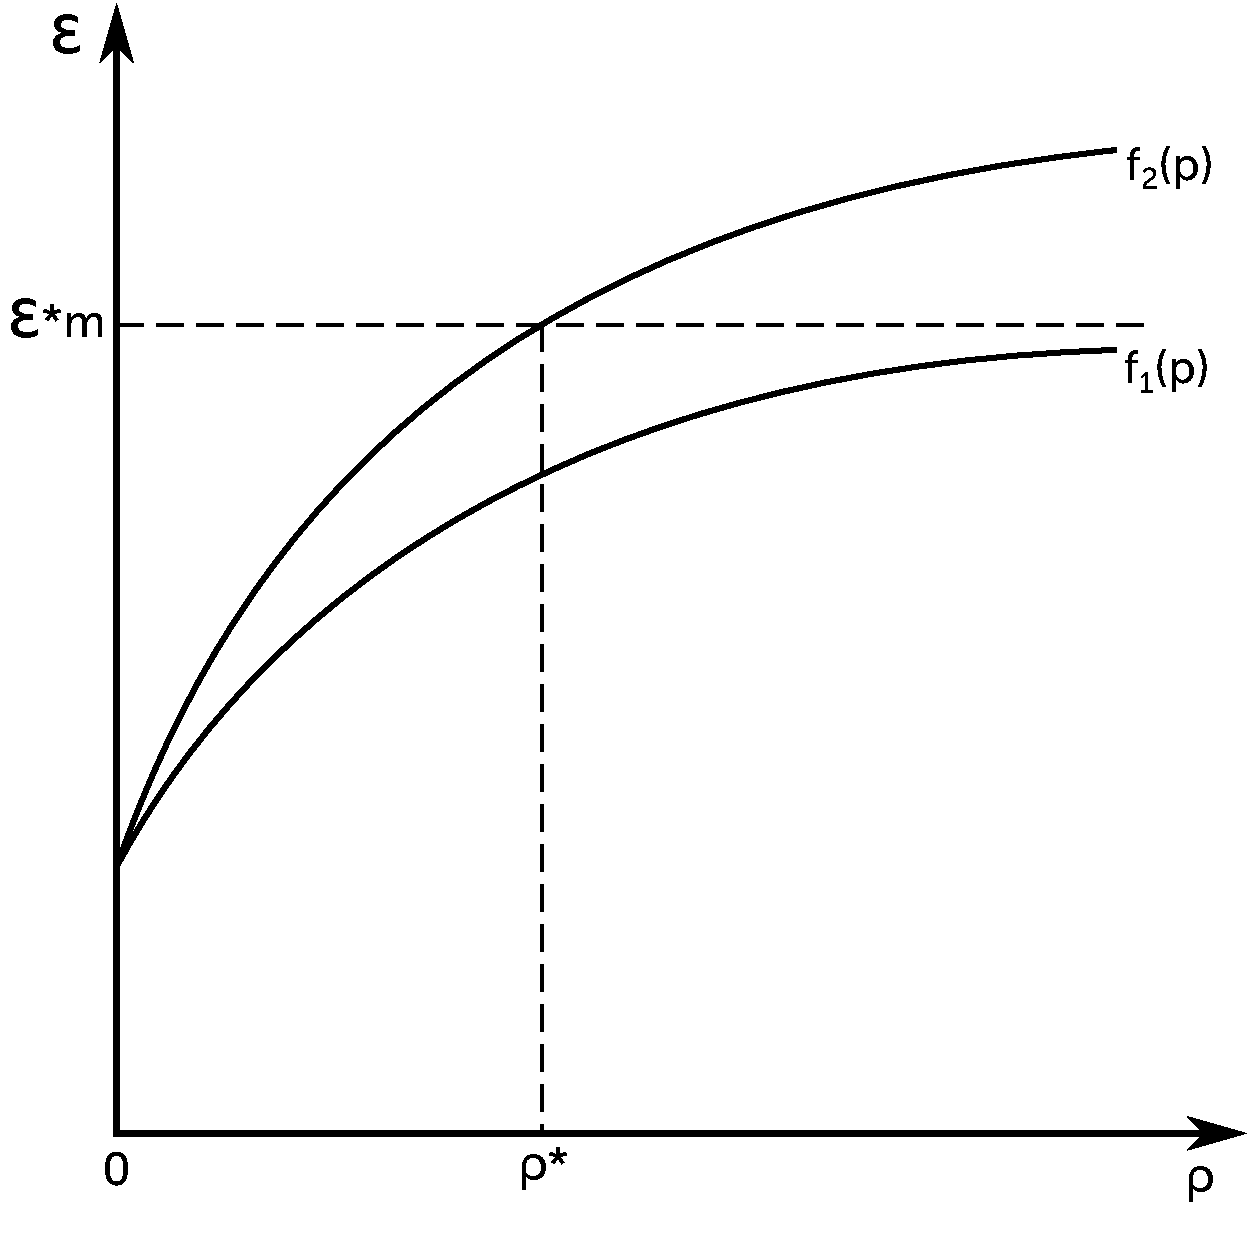
\includegraphics[width=8cm]{Graphics/graph1.pdf}
\caption{Evolution of $\varepsilon$, dependent on investment, $\rho$.}
\label{Fig:EpsilonEvolution}
\end{figure}

As artists do not bear the cost of DRM, they ideally require record
labels to invest the largest amount of money possible into DRM systems
in order to completely fight illegal piracy. On the other side, even
though firms still want to maximize their number of artists, $l_{F_{i}},$
even more so that the cost of DRM depends on it, they also bear the
cost of the investment and hence cannot choose an infinite amount
of investment.\\

Backward induction is once more used to solve this game. Several scenarios
are available. 
\begin{enumerate}
\item First of all, if $\varepsilon_{F_{i},max}<\varepsilon*,$ as presented
by $f_{1}(\rho)$ in figure \ref{Fig:EpsilonEvolution}, the record label $F_{i}$ will decide to not implement DRM systems.
\item If $\varepsilon_{F_{i},max}>\varepsilon*$, as described by $f_{2}(\rho)$
in figure \ref{Fig:EpsilonEvolution}, artists will want firms to enforce DRM systems, and two scenarios are possible.

% Sublist
\begin{enumerate}
\item If the distribution of artists is uniform across the four record labels
at the beginning of the game, such that $l_{F_{i}}=\frac{n}{4}$,
all firms could decide to implement DRM systems if the amount of investment
necessary to achieve $\varepsilon_{F_{i}}=\varepsilon^*$ does not overwhelm
the benefits of DRM. Otherwise, all firms decide to not implement
DRM in their albums. 
\item If the distribution of artists is not uniform, such that $l_{F_{1}}>l_{Fj},$$j=2,3,4$,$F_{1}$, for a same amount of investment necessary to achieve the critical
value of DRM effectiveness, could be the only firm able to implement
DRM systems. In this case, where the three other firms do not implement
DRM, $F_{1}$would catch all the artists, leaving the three other
record labels with a payoff of zero. This non-symmetric equilibrium
could have from one to four firms choosing to implement DRM systems. 
\end{enumerate}
\end{enumerate}

Formally, a given firm, $F_{i}$, would implement DRM systems iff:
\begin{eqnarray*}
\frac{\rho*}{l_{i}+1} & \geq & l_{i}((0.9+1.7\varepsilon_{F_{i},max})(\pi_{F_{i},A})+(0.95)(\pi_{F_{i},T}))\\
\pi_{m,DRM} & > & \pi_{m,\overline{DRM}}
\end{eqnarray*}

The other assumption about the effectiveness of DRM, namely the one
specifying that it is known by the firms and the artists, can also
put into question. It is indeed very likely that, back in the end
of the 1990s, record labels were unsure about the expected effect
these new protection systems would have on illegal piracy. From here
a new game with imperfect information can therefore be derived. For
simplicity, $\varepsilon$ is once more defined exogenously; nevertheless,
the effectiveness of DRM is no longer hold constant over time, as
described by the $\varepsilon_{t}$ curve in figure \ref{Fig:EpsilonEvolution}. The concavity
of the curve is due to (a) the increase of DRM effectiveness over
time - mainly thanks to investment in R\&D, even though $\varepsilon$
is in this model exogenous (b) the improve of consumers' knowledge
about how to pirate albums with DRM systems in it.\\

With this imperfect information, the game configuration changes. The
formal description of the game is provided in appendix \ref{Sec:FullGuessingGame}. Record labels
are still the first players to act, deciding whether or not implementing
DRM systems. However, while doing so, they do not know a priori the
actual value of $\varepsilon$, forcing them to first guess the estimation
of the parameters and then take a decision about DRM systems. The
firms' guessing process is presented in figure \ref{Fig:EpsilonGuessing}, as well as in appendix \ref{Sec:FullGuessingGame}.
The blue curve represents the actual effectiveness of DRM, in time
t. The green curve shows the firms' expectations based on obserations
about DRM effectiveness in t-1, so that $E(\varepsilon_{t}-\mu)=\varepsilon_{t-1}$.\\

Finally, the purple curve stands for the actual firms' expectations,
record labels being assumed to be optimistic about the impact of DRM
over illegal piracy - this overestimation of $\varepsilon$ being
represented by the parameters $\mu$. Followed this first step two
possible set of settings concerning the artists' beliefs and actions.
In the first one, artists completly trust the estimation of their
record label and, hence, based their choice of record labels on firms'
expectations about DRM effectiveness. The second configuration can
be a cheap talking game in which firms can lie about their estimated
expected $\varepsilon$ to attract more artists.\\

% Coloured epsilon graph.
\begin{figure}[h!]
\centering
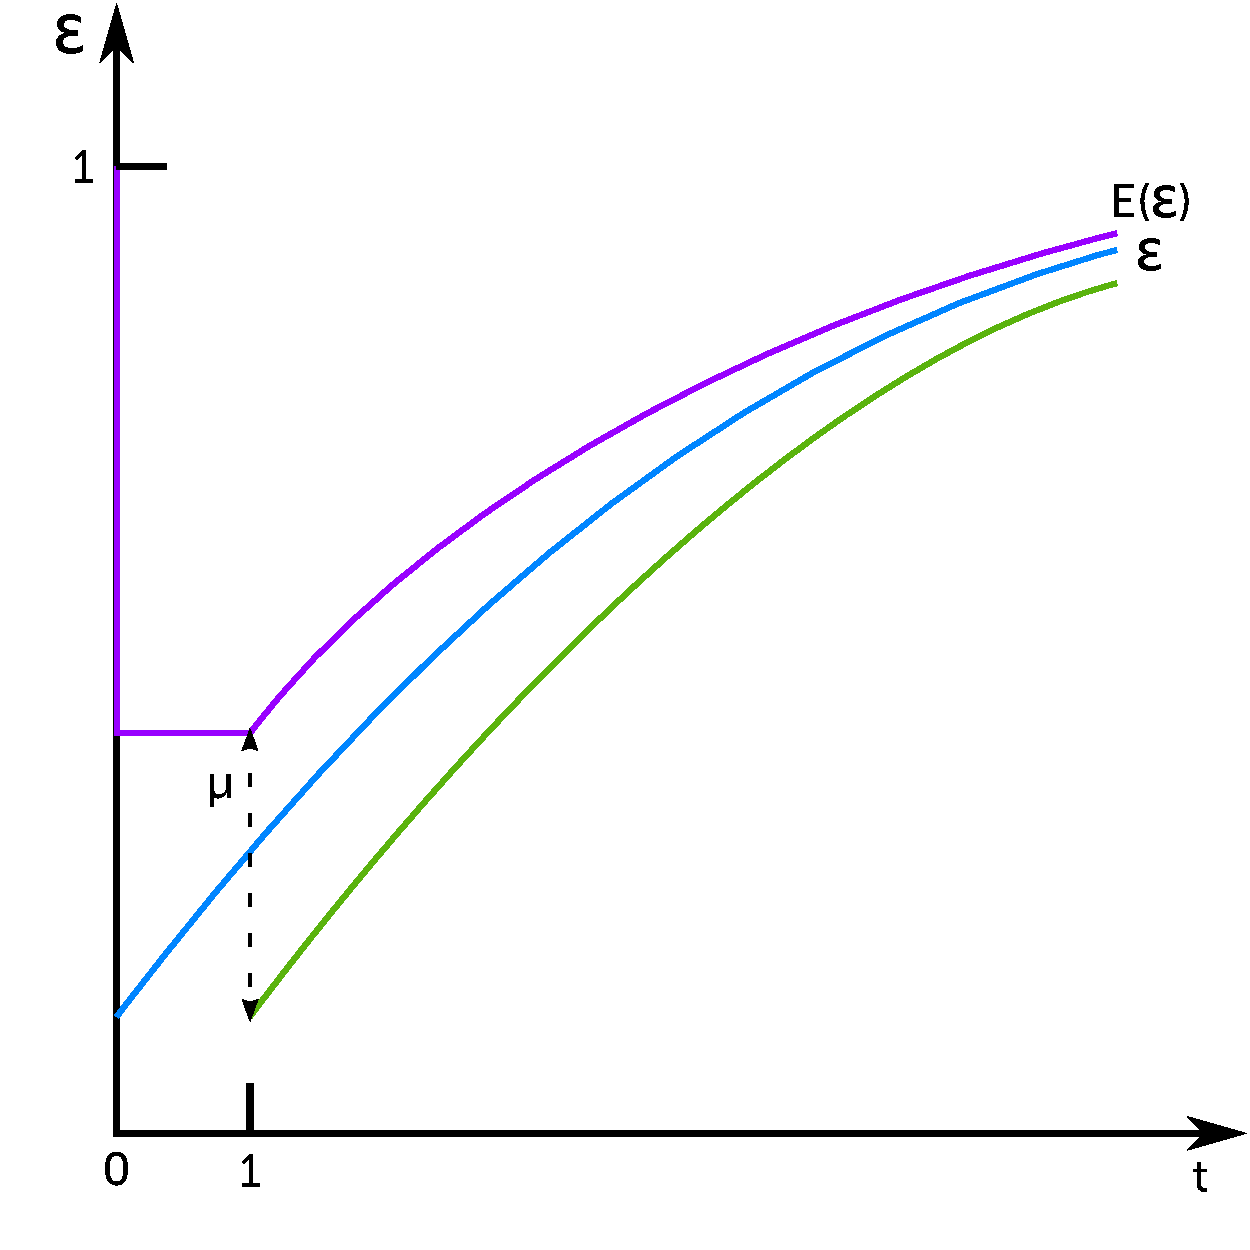
\includegraphics[width=8cm]{Graphics/graph2.pdf}
\caption{Evolution of $\varepsilon$, dependent on investment, $\rho$.}
\label{Fig:EpsilonGuessing}
\end{figure}

The insights about the solutions of the game presently analyzed only
concern the first configuration, without cheap talking. First of all,
if artists believe, at any time t, that $E(\varepsilon_{t})<\varepsilon*$,
$E(\varepsilon)$ being the expected impact of DRM on illegal piracy,
they would prefer choosing firms who have decided to not implement
DRM systems, and, ergo, no record labels will enforce DRM. If, however,
artists believe that $E(\varepsilon_{t})>\varepsilon*$, and that
for a sufficient period of time, record labels will be able to estimate
the shape of the $\varepsilon_{t}$curve. In this case, assuming uniform
distribution of the artist among the four firms, record labels will
either decide to enforce DRM systems in their product if the cost
of DRM is not too high, or, otherwise, decide not to go with DRM.\\

This game allows to study the timing with which record labels decide
to implement DRM. On one hand, as $\varepsilon$ increases over time,
a given firm, $F_{i}$, will have incentives to implement quickly
DRM if it expects its effect to be sufficiently important, because,
by doing so, $\varepsilon_{F_{i},t}>\varepsilon_{F_{j},t},$for $i\neq j.$On
the other hand, since firms do not know the actual impact of DRM and
are able to observe its effectiveness by observing firms' profits
which have implemented those systems, record labels also have incentives
to wait, even though their expectation about DRM effectiveness is
higher than the critical value of effectiveness required to increase
artists' profit. Specifically, if a given record label, $F_{i},$
is the only firm to use DRM, and $\varepsilon_{F_{i}}>\varepsilon*,$
as well as $E(\varepsilon_{F_{i}})\geq\varepsilon_{Fi}$, then all
the artists will sign contracts with $F_{i}$, such that$l_{F_{i}}=n$.
However, if $\varepsilon_{F_{i}}<\varepsilon*$, $F_{i}$ will lose
all its artists and will still have to bear the cost of DRM systems;
meanwhile, the other record labels will earn firm's artists without
paying any supplementary costs. The actual decision of a given firm
depends therefore on $E(\varepsilon_{F_{i}})$, $l_{i}$, $\rho$,
and the risk aversion of this given label.\\

Back in the late 1990s, record labels were so convinced that DRM systems
will help to fight effectively illegal download that they all decided
to implement those new quite unknown systems. Ten years later, they
realized that the actual effect of DRM systems were not that good,
and all firms abandoned DRM.

\section{Implications for the Video Game Industry}

In the video game industry, the use of DRM by publishers and acceptance of DRM by consumers has not reached an equilibrium at the time of writing. The medium of video games has some inherent qualities that make it a unique case. A large number of modern video games utilize the internet for play between multiple players. This process involves authenticating the copy of the game that a player is using and is a common way to combat illegal distribution.\\

Many games that have been released since the 1990's have been updated by their developers via internet downloaded \textit{patches}. These patches may add content or simply fix a performance issue with the game. In this way, most video games are not released as a final product, but as the first release of an ever-evolving product. To access this content, there is an authentication process like the one described above.\\

For many consumers, these two reasons are sufficient to render pirated copies too much of an inconvenience. In many cases, exclusively multiplayer games are not pirated by consumers who wish to play the game as intended. Proprietary media formats (such as all Nintendo optical discs) are also extremely effective deterrents of piracy. Yet video game piracy still remains constant within the industry.\\

Digitally distributed video games are released with an array of types of DRM that vary by the store through which the game is purchased, with some stores selling exclusively DRM-free copies of games. Even though this is a more complex scenario, we believe that our model will give insight into this situation.

\pagebreak

\bibliographystyle{plain}
\bibliography{References}

\pagebreak

\section{Appendix}

\subsection{Estimation of $\sigma_{A}$and $\sigma_{T}$}
\label{Sec:SigmaEstimates}

Recalling that the price elasticity of the album demand is 2.8\%,
$\sigma_{A}$, the variation in the quantity of album sold induced
by a one-unit variation in the album price, can be calculated through
the price-elasticity equation; formally,

\large
\begin{eqnarray*}
\left|\frac{\frac{a_{A} -\sigma_{A}(P'_{A})-(a_{A}-\sigma_{A}(P_{A}))}{a_{A}-\sigma_{A}(P_{A})}}{\frac{P_{A}'-P_{A}}{P_{A}}}\right|=\left|\frac{2.8}{100}\right|
\end{eqnarray*}
\normalsize

Solving for $\sigma_{A}$, with $\triangle P_{A}=1$, yields
\begin{eqnarray*}
\sigma_{A}=\left|\frac{2.8a_{A}}{97.2P_{A}}\right|
\end{eqnarray*}

The variation of album sold induced by a one-unit variation in the
album price depends therefore on the constant $a_{A}$, and on the
album price $P_{A}.$ Fixing $a_{A}$ equals to 100 allows to obtain
table \ref{Table:SigmaA}\footnote{
The weights are obtained by assuming that $P_{A}$ follows a normal distribution of mean 10 and standard deviation 2.5, $P_{A}\thicksim N(10,2.5)$
}. From here, the weighted average of $\sigma_{A}$ is 0.288, $\overline{\sigma_{A}}=0.288$.\\

The same method is used to estimate $\sigma_T$, the variation the number
of concert tickets sold following a one-unit variation in the concert
ticket price, knowing that the price elasticity of concert ticket
demand is almost inelastic, here quantifies as 0.5\%; formally:
\large
\begin{eqnarray*} 
\left|\frac{\frac{a_{T-\sigma_{T}(P'_{T})-(a_{T}-\sigma_{T}(P_{T}))}}{a_{T}-\sigma_{T}(P_{T})}}{\frac{P_{T}'-P_{T}}{P_{T}}}\right|=\left|\frac{0.5}{100}\right|
\end{eqnarray*}
\normalsize

Once more, solving for $\sigma_{T}$, with $\Delta P_{T}=1$, yields:
\begin{eqnarray*}
\sigma_{A}=\left|\frac{0.5a_{T}}{99.5P_{T}}\right|
\end{eqnarray*}

Finally, fixing $a_{T}=150$ allows to compute different values $\sigma_T$
depending on the price of a ticket, summarized in table \ref{Table:SigmaT}\footnote{
The weights are obtained by assuming that $P_{T}$ follows a normal distribution of mean 30 and standard deviation 25, $P_{T}\thicksim N(10,25)$
}. From here, the weighted average of $\sigma_{T}$ is 0.01, $\overline{\sigma_{T}}=0.01$.\\

\pagebreak

\begin{multicols}{2}
\begin{tabular}[h]{|c|c|c|}
\hline
$P_A$  & $\sigma_A$ & Weight \\ \hline
7 & -0.412 & 0.078 \\ \hline
7.5 & -0.384 & 0.097 \\ \hline
8 & -0.360 & 0.116 \\ \hline
8.5 & -0.339 & 0.133 \\ \hline
9 & -0.320 & 0.147 \\ \hline
9.5 & -0.303 & 0.156 \\ \hline
10 & -0.288 & 0.160 \\ \hline
10.5 & -0.274 & 0.156 \\ \hline
11 & -0.262 & 0.147 \\ \hline
11.5 & -0.250 & 0.133 \\ \hline
12 & -0.240 & 0.116 \\ \hline
12.5 & -0.230 & 0.097 \\ \hline
13 & -0.222 & 0.078 \\ \hline
13.5 & -0.213 & 0.060 \\ \hline
14 & -0.206 & 0.044 \\ \hline
14.5 & -0.199 & 0.032 \\ \hline
15 & -0.192 & 0.022 \\ \hline
\end{tabular}
\captionof{table}{Values used to estimate $\sigma_A$.}
\label{Table:SigmaA}

\columnbreak

\begin{tabular}[h]{|c|c|c|}
\hline

$P_T$ & $\sigma_T$ & Weight \\ \hline
10 & -0.075 & 0.012 \\ \hline
15 & -0.050 & 0.013 \\ \hline
20 & -0.003 & 0.015 \\ \hline
25 & -0.003 & 0.016 \\ \hline
30 & -0.002 & 0.016 \\ \hline
35 & -0.002 & 0.016 \\ \hline
40 & -0.002 & 0.015 \\ \hline
45 & -0.001 & 0.013 \\ \hline
50 & -0.001 & 0.012 \\ \hline
55 & -0.001 & 0.010 \\ \hline
60 & -0.001 & 0.008 \\ \hline
65 & -0.001 & 0.006 \\ \hline
70 & -0.001 & 0.004 \\ \hline
75 & -0.001 & 0.003 \\ \hline
80 & -0.001 & 0.002 \\ \hline
90 & -0.001 & 0.001 \\ \hline
100 & -0.001 & 0.000 \\ \hline
\end{tabular}
\captionof{table}{Values used to estimate $\sigma_T$.}
\label{Table:SigmaT}
\end{multicols}

\pagebreak

\subsection{Formal Description of the DRM Game with\\
Imperfect Information} \label{Sec:FullGuessingGame}

Recalling that record labels' profit in period t is described by the
following equation:
\begin{eqnarray*}
\pi_{F_{i},t}=l_{i}((1+\delta(1.7\varepsilon_{t}-0.1))(\pi_{F_{i},A})+(1-\delta0.05)(\pi_{F_{i},T}))-\delta(\frac{\rho}{l_{i}+1})
\end{eqnarray*}

This payoff function can be adapted to the new configuration game
in which record labels, and artist, do not know the actual value of
$\varepsilon$. Therefore, when a given firm, $F_{i},$ has to decide
whether or not implementing DRM in its albums, it does not consider
its profit but its expected profit given the expected effectiveness
of DRM; formally:
\begin{eqnarray*}
E(\pi_{F_{i},t})=l_{i}((1+\delta(1.7E(\varepsilon_{F_{i},t})-0.1))(\pi_{F_{i},A})+(1-\delta0.05)(\pi_{F_{i},T}))-\delta(\frac{\rho}{l_{i}+1})
\end{eqnarray*}

In the situation where artists fully trust record labels about the
expected impact of DRM on illegal download, such that $E_{F_{i}}(\varepsilon_{t})=E_{m}(\varepsilon_{t})$, artists' expected payoffs is defined similarly.
\begin{eqnarray*}
E(\pi_{m,t})=(1+\delta(1.7E(\varepsilon_{F_{i},t})-0.1))(\pi_{m,A})-C_{A}+(1-\delta0.05)(\pi_{m,T})-C_{T}
\end{eqnarray*}

The equation given the expectation about the DRM effectiveness is
founded on the rational expectation theory, with some adjustments.
Specifically, in the first period t,firms are really optimist about
the impact of DRM systems on illegal download, such that $E_{F_i}(\varepsilon)=1$.\\

After the first period, firms based their expectations on what they
observe in previous periods; however, firms are also assumed to be
optimistic about the effect of DRM - which can also translate the incentive
they have to overestimate $\varepsilon$ in order to convince artists
to sign a contract with them. Hence, firms' expectations after the
first period are:
\begin{eqnarray*}
E_{F_{i}}(\varepsilon_{t+1})=\varepsilon_{F_{i},t} + \mu
\end{eqnarray*}

with
\begin{eqnarray*}
\varepsilon_{F_{i},t}=E_{F_{i}}(\pi_{F_{i},t})-\pi_{F_{i},t}=-\frac{E_{F_{i}}(\pi_{F_{i},t})-\pi_{F_{i},t}}{1.7P_{A,F_{i}}}+E_{F_{i}}(\varepsilon)
\end{eqnarray*}

Finally, expectations are assumed to be more and more close to
the actual value of $\varepsilon$ since record labels accumulated
data over time and are able to distinguish the shape of the $\varepsilon$
curve; formally, $\lim_{t\rightarrow\infty}E_{F}{}_{i}(\varepsilon_{t})-\varepsilon_{t}=0$.\\

All those assumptions about the firms' and artists' beliefs are shown
in section \ref{Sec:Extensions}, figure \ref{Fig:EpsilonGuessing}. Insights about solutions for this game are
also presented in this previous section.

\end{document}